\clearpage

\def\chaptertitle{System Implementation}

\lhead{\emph{\chaptertitle}}

\chapter{\chaptertitle}
\label{ch:experimental-setup}

Based on the previous high-level overview of the architectures and algorithms involved, in this chapter, we will first discuss the micro-service application architecture used to test the algorithm, along with its features in section \ref{sec:ch4-microservice-overview}. Based on this, section \ref{sec:ch4-data-generation} will give an explanation of the workload generator bundled along with the micro-service deployment, and how that is used to generate the time-series workload typically seen in edge architectures. Finally, we will discuss the technical configurations of the hybrid autoscaler itself in section \ref{sec:ch4-hybrid-auto-arch}. This will involve how the workload information is communicated between cloud and edge layers, how the autoscaler parameters for both reactive and proactive subsystems are configured, and how the forecaster is configured to use the time-series data to generate forecasted values for a sufficiently large time-period.

\section{Microservice Overview}
\label{sec:ch4-microservice-overview}

DeathStarBench \footnote{\url{https://github.com/delimitrou/DeathStarBench/tree/master/socialNetwork}}, a social media micro-service developed by Y. Gan et al. \cite{gan2019open} is ideal for benchmarking SLA-compliance, and was thus deployed on Kubernetes. The application mimics a large-scale social network application and supports common actions such as registering and login for user credentials, creating user posts on their timeline, reading other user timelines, receiving follower recommendations, following and unfollowing of other users, and searching for users or posts. Figure \ref{fig:social-network-arch} shows the architecture of the micro-service.\par

\begin{figure}[htb]
    \centering
    \caption{DeathStarBench Social-Network Architecture, courtesy Y. Gan et al. \cite{gan2019open}}
    \label{fig:social-network-arch}
    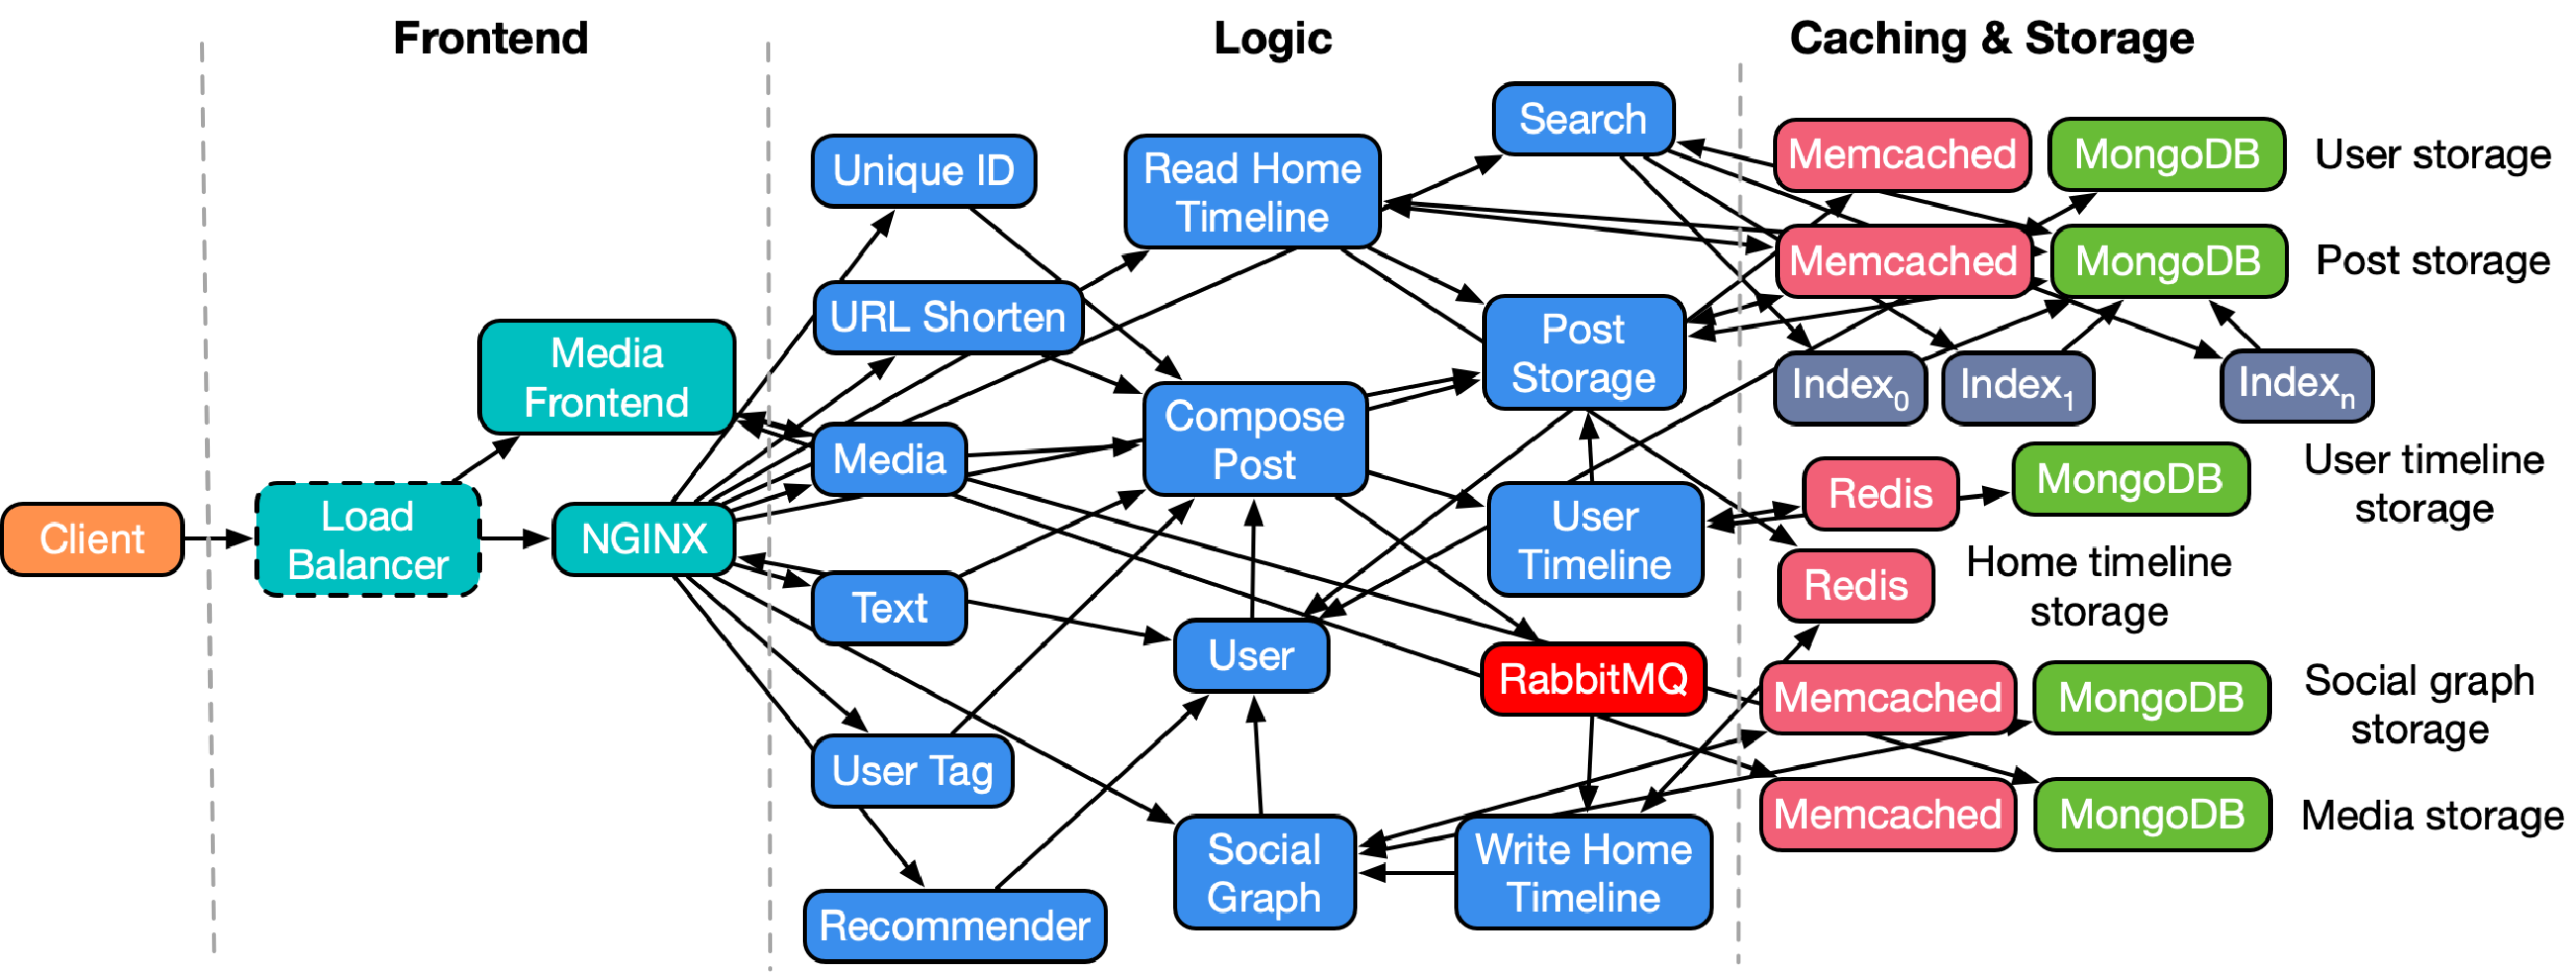
\includegraphics[width=1.0\linewidth]{Figures/Social-Network-Architecture.pdf}
\end{figure}

The end-to-end service implementation depicts a social network with a broadcast style approach. The user or client sends requests using HTTP to the front-end layer. These requests are processed using a load balancer implemented using an open-source deployment known as NGINX \footnote{\url{https://nginx.org/en/}}. NGINX then specifies the web server that has been selected, and communicates with the micro-services in the logic layer, which are responsible for composing and displaying the user and timeline posts. The logic layer also consists of micro-services for serving advertisements, search engines, and other capabilities commonly found in large scale applications. The search and advertisement engines are machine learning plugins capable of serving recommendations based on user interactions. The logic layer is capable of handling posts containing text, links, and media. Users can also mark other user's posts as favourites, re-post them, and reply to them privately or publicly. Users can also follow, unfollow, or block others. All these interaction results are stored in the storage layer, which uses memcached for caching results, and MongoDB for storing user profiles, posts, media, and recommendations in a persistent manner.

Users can sign in to the application website by connecting to the user interface deployment, which can be assigned a DNS address. For simplicity, in this experiment the Kubernetes node IP address was exposed through the deployment, along with the social media application port. For example, an API request for reading user timelines will look as follows:\par

\begin{lstlisting}[
  caption={Social network API call template},
  captionpos=t,
  label={lst:social-network-api-template},
]
http://<node-IP>:<app-port>/wrk2-api/user-timeline/read
\end{lstlisting}

\section{Data Generation}
\label{sec:ch4-data-generation}

The social media deployment also comes with an HTTP workload generator, which
is leveraged to create a realistic simulation of a typical day of workload for the microservice application. The generator, known as ``wrk2'', is an open-loop load generator. HTTP requests are sent out according to the user configuration, regardless of whether or not the responses of the previous requests have been received. This avoids issues such as queuing delays in the server, helping to maintain an even load throughout the generation process which aids in benchmarking. The workload generator supports a variety of load generation use-cases, as well as different APIs. For example, a POST request with a total load generation of 8 requests per second, using 2 parallel threads, with 5 open HTTP connections, and for a duration of 30 seconds looks as follows:\par

\begin{lstlisting}[
  caption={Workload generation example},
  captionpos=t,
  label={lst:workload-gen-example},
  language=bash
]
$ wrk2 -t2 -c5 -d30 -R8 http://<node-IP>:<app-port>/wrk2-api/post/compose
\end{lstlisting}



A typical IoT application in the edge has a semi-predictable workload pattern. In this experiment, it is assumed that the workload peaks in the morning and evening, while seeing moderate usage during the afternoon. The workload is lowest at night. The workload simulator was modified to introduce an element of randomness to mimic realistic weekly workloads, which can vary on occasions such as weekends and public holidays.\par

To achieve this, an IoT workload algorithm was created for leveraging the wrk2 generator to achieve this time-series. This is explained in algorithm \ref{alg:work-gen}. A constant light workload is set for night time consisting of six hours between 12:00am and 06:00 am, while different workloads for the eighteen different day time hours are set, with peaks set in the morning and evening, and dips in the afternoon. The algorithm also contains a small random ``offset'' variable to depict the randomness inherent in the workload. This is depicted using the function $\mathcal{U}$, where $\mathcal{U}(0,1)$ returns a random number between 0 and 1. This workload is then executed using the wrk2 generator to apply the HTTP load on the microservice.

%TC:ignore
\begin{algorithm}
    \caption{IoT workload generation algorithm}
    \label{alg:work-gen}
    \begin{algorithmic}
        \State $offset \gets \alpha$
        \State $night\_workload \gets \omega$
        \State $day\_workload \gets [ \delta_1, \delta_2, ... , \delta_{18}]$
        \While{True}
            \For {i $\leftarrow$ 0 ... 6}
                \State $result \gets generate(night\_workload + \mathcal{U}(-offset,offset)$
            \EndFor
            \For {i $\leftarrow$ 0 ... 18}
                \State $result \gets generate(day\_workload[i] + \mathcal{U}(-offset,offset)$
            \EndFor
        \EndWhile
    \end{algorithmic}
\end{algorithm}
%TC:endignore

\section{Hybrid Autoscaler Configuration}
\label{sec:ch4-hybrid-auto-arch}

\suhrid{Move all algorithm pseudo-code to ch3, move lstm justification to ch3, all code implementation should remain here \cmark}

In this section, the configuration parameters of the proposed hybrid autoscaler will be discussed. First, a brief background will be provided of how the social network application is connected to Kubernetes, so that it can send default and custom metrics such as application CPU usage and latency respectively. These custom metrics will then be discussed further, and how they are integrated for use in the horizontal pod autoscaler.\par

With this background, a further discussion of the reactive subcomponent of the hybrid autoscaler is conducted, explaining its parameters and how it connects to the custom metrics API. The details of the proactive autoscaler are then discussed. This includes the architecture of the LSTM, default hyper-parameters, and the lookback and forecasting window. Finally, the autoscaler heuristic feedback will be discussed, including the exact parameters it modifies when it discovers an SLA violation.\par

\subsection{Custom Metrics Export To Kubernetes}
\label{subsec:metrics-export}

The social media application comes bundled with Jaeger \footnote{\url{https://www.jaegertracing.io/}} deployment. Jaeger is an open-source distributed tracing platform, capable of tracking several application metrics of each network request and per-microservice request, and stores them in a centralized database. One such metric is the details of API latency for the application. The latency information is extremely detailed, and is broken down per each deployment in the social media architecture as defined by Figure \ref{fig:social-network-arch}. Alongside the latency breakdown, Jaeger can automatically generate graphs of the Kubernetes deployments which are utilized by API calls. This is particularly useful for identifying deployment bottlenecks which are prime targets for autoscaling.\par

Before this latency information can be useful in the autoscaling solution, it must be imported to Kubernetes in a readable format. This was achieved through the use of a tool called Prometheus. Prometheus \footnote{\url{https://prometheus.io/docs/introduction/overview/}} is an open-source deployment used for monitoring applications. Prometheus consists of a multi-dimensional data model for storing time-series data through key/value pairs, a custom built querying language known as PromQL, which is used to leverage and search through this data model, and a graphing and dashboard user interface to aid in visualization. Due to the heavy nature of the deployment, Prometheus must be deployed on the cloud layer.\par

%TC:ignore
\begin{lstlisting}[
  caption={Jaeger-Scraper server},
  captionpos=t,
  label={lst:jaeger-scraper},
  float=ht
]
const avg_counter = new Gauge({
        name: 'wrk2_avg_api_latency',
        help: 'Jaeger average post API latency (ms)'
});

get('/metrics', async (req, res) => {
    let url = process.env.JAEGER_URL;
    const data = await axios.get(url);
    let avg_duration = 0;

    let durations = data.map(components => {
        let duration = components.duration;
        return duration;
    });

    avg_duration = durations.reduce( (a,b) => a+b ) / durations.length;
    avg_counter.set(avg_duration);

    result.set('Content-Type', avg_counter);
});
\end{lstlisting}
%TC:endignore

To facilitate the export of Jaeger metrics to Prometheus, a custom deployment was created which scrapes these metrics at a given time interval, and pushes it to Prometheus. The deployment, which was named ``Jaeger-Scraper'', was a JavaScript express server set up on Kubernetes using Docker, and the server code was as shown in listing \ref{lst:jaeger-scraper}. The server uses the open source NPM library ``prom-client''\footnote{\url{https://github.com/siimon/prom-client}} to create a Prometheus Gauge. A gauge is an extension of the Prometheus metric counter, the primary difference being that it can be both increased or decreased, whereas the counter can only be incremented. When the metrics API endpoint is called, the scraper gets the latest Jaeger metrics within a fixed window, and calculates the average latency of the time period. This value is then ready to be pushed to the Prometheus database.

Once this server is deployed on the Kubernetes cloud layer, a service-monitor for Prometheus is written, which tells Prometheus to invoke the GET API this server exposes at a set interval of time. It is through this API call that the latency value gets pushed to the Prometheus database. By default, the service-monitor calls the $/metrics$ endpoint, which is what the Jaeger-Scraper is configured with. For this thesis, this interval was set at 15 seconds, and the configuration is shown in listing \ref{lst:jaeger-scraper-svc-monitor}.

%TC:ignore
\begin{lstlisting}[
  caption={Jaeger-Scraper service monitor},
  captionpos=t,
  label={lst:jaeger-scraper-svc-monitor},
  float=ht
]
apiVersion: monitoring.coreos.com/v1
kind: ServiceMonitor
metadata:
  labels:
    app: jaeger-scraper
  name: jaeger-scraper-svc-monitor
spec:
  endpoints:
  - interval: 15s
    port: http
  selector:
    matchLabels:
      app: jaeger-scraper
\end{lstlisting}
%TC:endignore

The scraped values are now visible when querying the metrics endpoint, and listing \ref{lst:jaeger-scraper-metric} below shows an example of how the metrics are displayed. However, while the latency metrics are now present in Prometheus, the next step is to import these metrics to the Kubernetes custom metrics server.\par

%TC:ignore
\begin{lstlisting}[
  caption={Jaeger-Scraper metrics collector},
  captionpos=t,
  label={lst:jaeger-scraper-metric},
  float=ht
]
$ curl $(kubectl get service jaeger-scraper --template \
'{{.spec.clusterIP}}'):8081/metrics
# HELP wrk2_avg_api_latency Jaeger average post API latency (ms)
# TYPE wrk2_avg_api_latency gauge
wrk2_avg_api_latency 0
\end{lstlisting}
%TC:endignore

By default, Kubernetes autoscaling can scale resources based on CPU and memory utilization. However, for more complex use-cases, more metrics need to be taken into account to make such decisions. To aid in this process, the Prometheus Adapter \footnote{\url{https://github.com/kubernetes-sigs/prometheus-adapter}} was created to leverage the metrics collected and stored by the Prometheus deployment, and feed them to Kubernetes. These metrics are exposed via an API service and are consumed by the hybrid autoscaler for decision making.\par

%TC:ignore
\begin{lstlisting}[
  caption={Prometheus adapter configmap},
  captionpos=t,
  label={lst:prometheus-adapter-configmap},
  float=ht
]
apiVersion: v1
kind: ConfigMap
metadata:
  name: custom-metrics-prometheus-adapter
data:
  config.yaml: |
    rules:
    - seriesQuery: wrk2_avg_api_latency{namespace!=""}
      resources:
        template: <<.Resource>>
      name:
        as: ${1}
        matches: ^(.*)
      metricsQuery: <<.Series>>
\end{lstlisting}
%TC:endignore

The prometheus adapter requires a configuration map (ConfigMap) to translate Prometheus metrics to Kubernetes custom metrics. The adapter does so in four steps.

\begin{itemize}
    \item Discovery - The adapter discovers the metrics available in Prometheus.
    \item Association - Figure out the association between each metric and Kubernetes resource.
    \item Naming - Assigns a name to these resources through which the custom metrics API can expose them.
    \item Querying - Queries the Prometheus deployment to get the actual metric numbers.
\end{itemize}

The hybrid autoscaler requires the default CPU metric, as well as the custom latency metric. Thus we define these this additional metric for configuring in Kubernetes. Listing \ref{lst:prometheus-adapter-configmap} shows the discovery, association, naming, and querying steps to do so. In the ``config.yaml'', the ``seriesQuery'' corresponds to discovery, ``resources'' to association, ``name'' to naming, and ``metricsQuery'' to querying.

%TC:ignore
\begin{lstlisting}[
  caption={Custom metrics API example},
  captionpos=t,
  label={lst:custom-metrics-example},
  float=ht
]
$ kubectl get --raw /apis/custom.metrics.k8s.io/v1beta1 | jq .
{
  "groupVersion": "custom.metrics.k8s.io/v1beta1",
  "resources": [
    {
      "name": "services/wrk2_avg_api_latency",
      ...
    },
    {
      "name": "pods/wrk2_avg_api_latency",
      ...
    },
    {
      "name": "namespaces/wrk2_avg_api_latency",
      ...
    }
  ]
}
$ kubectl get --raw \
/apis/custom.metrics.k8s.io/v1beta1/namespaces/default\
/services/*/wrk2_avg_api_latency_per_minute | jq .
{
  "kind": "MetricValueList",
  "apiVersion": "custom.metrics.k8s.io/v1beta1",
  "items": [
    {
      "metricName": "wrk2_avg_api_latency",
      "value": "0"
      ...
    }
  ]
}
\end{lstlisting}
%TC:endignore

Now, the Kubernetes custom metrics API exposes the following additional APIs under the resources pods, services and namespaces as shown in listing \ref{lst:custom-metrics-example}. Alongside this, querying individual metrics gives resource values which will be used for autoscaling purposes.

\subsection{Reactive Autoscaler}
\label{subsec:reactive-auto-subsection}

With the custom metrics now being exposed by Kubernetes, all the tools required for the reactive auto-scaling subsystem are in place. This will be built as an extension of the default Kubernetes horizontal pod autoscaler.\par

As discussed in subsection \ref{subsec:ch3-hybrid-arch}, the reactive autoscaler must be set to a value that is not too small or large. For this experiment, the parameters of the autoscaler were modified by setting both the cooldown values to 15 seconds, or one control loop, and maintain the toleration value at the default. This ensures that reactive autoscaling occurs as quickly as possible, to minimize SLA violations, while decreasing the chances of resources constantly being scaled up and down in a yo-yo manner \cite{sides2015yo}. Listing \ref{lst:reactive-cooldown-config} shows the configuration changes to achieve this.\par

%TC:ignore
\begin{lstlisting}[
  caption={Reactive autoscaler cooldown configuration},
  captionpos=t,
  label={lst:reactive-cooldown-config},
  float=ht
]
spec:
  behavior:
    scaleDown:
      policies:
      - periodSeconds: 15
        type: Pods
      stabilizationWindowSeconds: 15
    scaleUp:
      policies:
      - periodSeconds: 15
        type: Pods
      stabilizationWindowSeconds: 15
\end{lstlisting}
%TC:endignore

While these parameters are configurable by other users, experimental results showed that for SLA-compliant applications, these parameters were capable of producing the best results for a wide array of use-cases. Higher cooldown windows lead to SLA-violations due to the time taken to scale resources, while smaller windows caused the constant scaling up and down of resources on small variations, leading to a loss of resource availability and increased deployment costs for the entire architecture.

\subsection{Proactive Autoscaler}
\label{subsec:ch4-proactive-auto-subsection}

\suhrid{Move this to ch4, move hyper-parameter tuning to ch4 \cmark}

\suhrid{TODO: In the proactive config, note how there is a callback which stops the training if loss doesn't reduce for 10 iterations. This is done to prevent over-fitting as demonstrated by Siami-Namini et al. \cite{siami2018comparison} \cmark}

The proactive autoscaler has a Kubernetes configuration that is similar to the reactive one shown in listing \ref{lst:reactive-cooldown-config}. The same cooldown values of 15 seconds are applied here as well, to keep it consistent with the reactive solution.\par

The proactive algorithm \ref{alg:proactive-forecast-alg} was deployed on Kubernetes using the same method as the Jaeger-Scraper, and was accessible in the edge network by invoking a GET API. However, to capture the $forecasted\_cpu$ metric returned by the forecaster in the custom API, the Prometheus Adapter configuration map required to be modified to append the value, as shown in listing \ref{lst:prometheus-adapter-configmap-proactive}. With this addition, the proactive autoscaler was able to receive forecasted values.\par

%TC:ignore
\begin{lstlisting}[
  caption={Prometheus adapter configmap},
  captionpos=t,
  label={lst:prometheus-adapter-configmap-proactive},
  float=ht
]
- metricsQuery: <<.Series>>
  name:
    as: ${1}
    matches: ^(.*)
  resources:
    template: <<.Resource>>
  seriesQuery: forecasted_cpu{namespace!=""}
\end{lstlisting}
%TC:endignore

The forecaster was a deep-learning machine learning model, which consists of three LSTM layers, alternated with two dropout layers. These dropout layers were used to prevent data over-fitting. Finally, the last layer was a densely connected neural-network which generated the forecaster output in the required shape. For this experiment, the output was 540 data points, which was approximately the amount of data required to forecast 24 hours of workload. Table \ref{tab:lstm-layers} shows the detailed information about the forecaster model layers.\par

%TC:ignore
\begin{table}
    \caption{Overview of proactive forecaster layers.}\label{tab:lstm-layers}
    \centering
    \begin{tabular}{|l|l|l|}
        \hline
        Layer Details & Output Shape & Parameter Count\\
        \hline
        $LSTM_{1}$ & (10, 50) & 10400\\
        $Dropout_{1}$ & (10, 50) & 0\\
        $LSTM_{2}$ & (10, 50) & 20200\\
        $Dropout_{2}$ & (10, 50) & 0\\
        $LSTM_{3}$ & (50) & 20200\\
        $Dropout_{3}$ & (50) & 0\\
        $Dense_{1}$ & (540) & 27540\\
        \hline
    \end{tabular}
\end{table}
%TC:endignore

\suhrid{Talk about the actual data generated by the workload algo, how savgol smooths data beforehand, how data is normalized before training, lstm default epoch, learn rate etc params, graphs from tensorboard, final graph of actual and predicted data and how it accurately predicts the beginning of the peaks even though the rest may not be as accurate. \cmark}

The data which was generated by the workload algorithm \ref{alg:work-gen} was periodically scraped and stored by the autoscaler daemon. An example of how this data may look over a period of four days is shown in figure \ref{fig:lstm-init-data}.

\begin{figure}[htb]
    \centering
    \caption{Example of generated workload}
    \label{fig:lstm-init-data}
    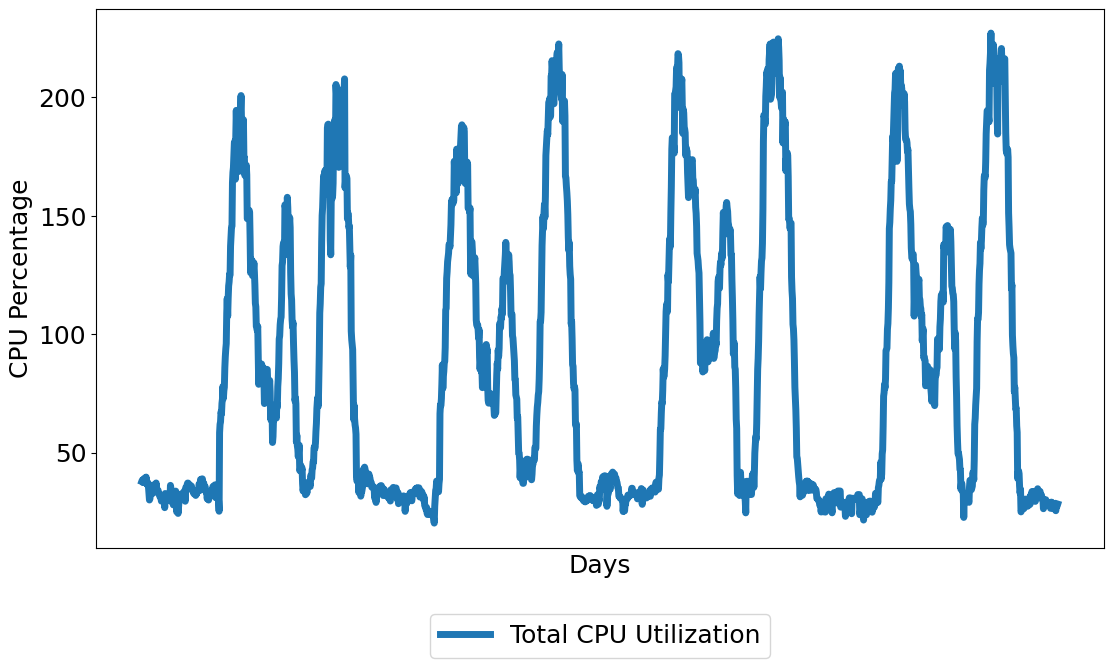
\includegraphics[width=1.0\linewidth]{Figures/LSTM-Initial-Data.png}
\end{figure}

This data has two major peaks during the morning and evening, with one smaller peak in the afternoon. The night time workload is consistently minimal. Due to the randomness included in the algorithm, each of the peaks are never the exact same, which helps mimic the real data an edge architecture would experience. However, this data has several abrupt changes every few minutes, for example the utilization could be 100\% at 5:00pm, then suddenly drop down to 75\% at 5:10pm, before coming back up to 110\% at 5:20pm. These abrupt changes makes it difficult for the LSTM to be able to accurately predict the future workloads, and requires a much larger input sequence to reduce model loss, which can significantly drive up training times.\par

To get around this issue, the proactive autoscaler introduces a data pre-processing component. This involves the use of noise reduction and data smoothing algorithm. This is done through a popular technique known as the Savitzky-Golay filter \cite{savitzky1964smoothing}. This filter takes $N$ points in a given time-series, with a filter width $w$, and calculates a polynomial average of order $o$ \cite{schafer2011savitzky}. The resulting time-series data which can be seen in figure \ref{fig:lstm-smooth-data} has considerably less deviations between consecutive points, and devoid of noise.\par

\begin{figure}[htb]
    \centering
    \caption{Example of pre-processed workload}
    \label{fig:lstm-smooth-data}
    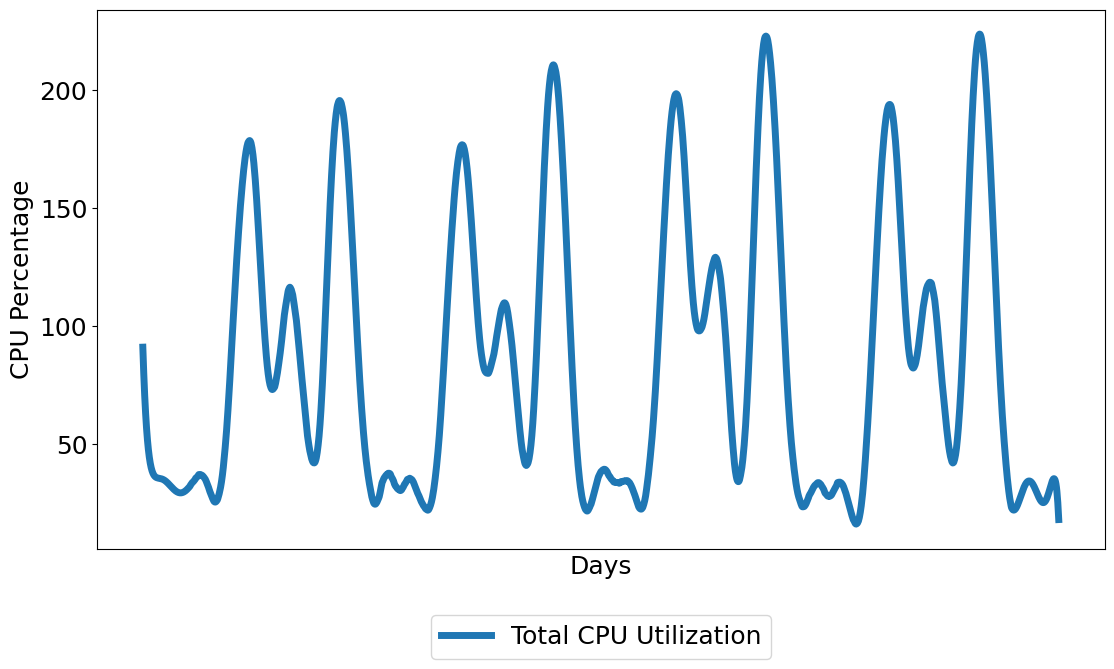
\includegraphics[width=1.0\linewidth]{Figures/LSTM-Smooth-Data.png}
\end{figure}

The filtered data is then normalized, and is then ready to be used to trained the model. Alongside the architecture configured in table \ref{tab:lstm-layers}, the LSTM model contains the following default hyper-parameter values depicted in table \ref{tab:lstm-params}.

%TC:ignore
\begin{table}
    \caption{Proactive forecaster hyper-parameter values.}\label{tab:lstm-params}
    \centering
    \begin{tabular}{|l|l|l|}
        \hline
        Hyper-parameter & Value\\
        \hline
        $learning\_rate$ & 0.005\\
        $epochs$         & 75\\
        $batch\_size$    & 100\\
        $optimizer$      & Adam \cite{diederik2014adam}\\
        \hline
    \end{tabular}
\end{table}
%TC:endignore

The parameters are chosen in such a way that they minimize training time and over-fitting, while maximizing prediction accuracy. To further reduce over-fitting, an additional function known as ``early-stop'' is defined which halts the training of the model if the loss does not decrease for 10 consecutive epoch iterations. These parameters were determined based on the research experiments conducted by Siami-Namini et al. \cite{siami2018comparison}.\par

The model training, validation and comparison with previous model performances takes approximately 3 minutes, after which, the model predicts the subsequent day's forecast. Figure \ref{fig:lstm-final-data} shows how this looks. The forecaster accurately depicts the initial peaks for the entire day. However, the rest of the data may not be as accurate, however this is not a significant drawback for the hybrid model, as the reactive algorithm is capable of making minor adjustments.

\begin{figure}[htb]
    \centering
    \caption{Example of the forecasted workload}
    \label{fig:lstm-final-data}
    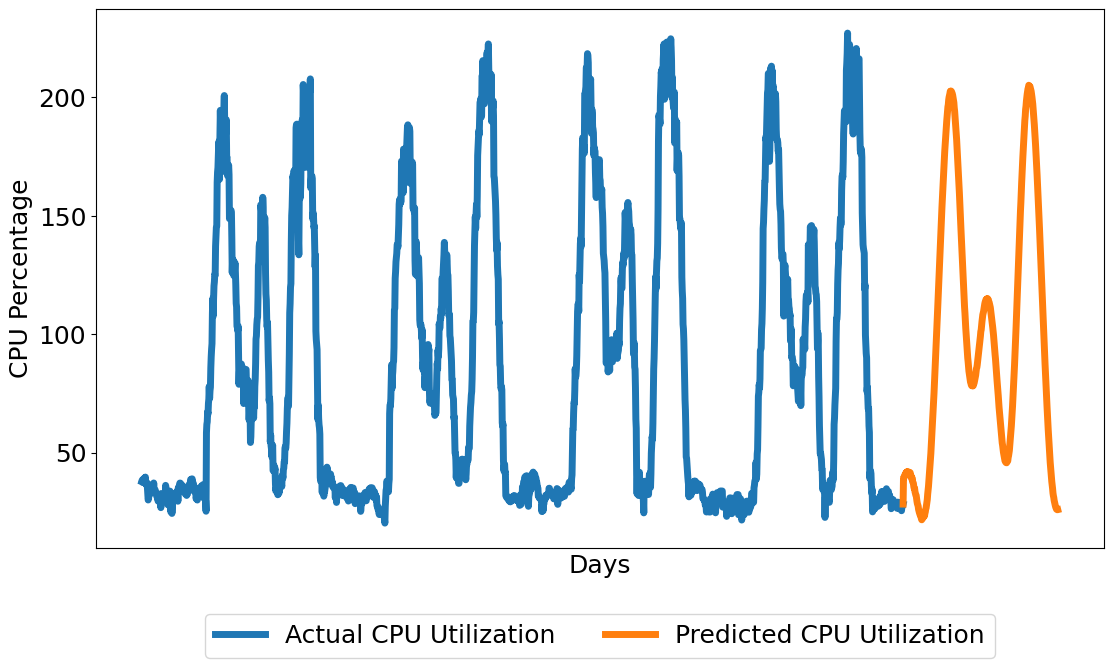
\includegraphics[width=1.0\linewidth]{Figures/LSTM-Final-Data.png}
\end{figure}

\subsection{Autoscaler Daemon}
\label{subsec:ch4-auto-daemon-subsection}

The autoscaler daemon stores a maximum of seven days of data for use by the proactive forecaster. Data that is too old is not very useful for a time-series model training on semi-predictable data \cite{greff2016lstm}, and only increases training time without adding much to the accuracy. This data is refreshed every 15 seconds to ensure that the latest data is always available to the hybrid autoscalers.\par

The daemon sends a training request to the proactive autoscaler once every night. The time is chosen so that, due to the low resource usage, the training process can claim as much of the edge resources as possible without affecting the network availability. However, before sending the request, the daemon computes whether or not an SLA violation took place in the past 24 hours or not. If it detects a violation, it assumes that the forecaster has not learnt enough of the time-series due to a variety of reasons such as lack of training data or conservative parameter values. To counteract this, the daemon performs the following corrections:

\begin{itemize}
    \item $learning\_rate$ is decreased by 0.0005, to a minimum value of 0.002.
    \item $epochs$ is increased by 5, to a maximum of 100.
    \item $batch\_size$ is increased by 10, to a maximum of 200.
    \item $early\_stop$ threshold is increased by 5, to a maximum of 25.
\end{itemize}

The assumption here is the training accuracy can be kick started by sacrificing training time for one duration to better learn the time series features and thus reduce SLA violations. As long as SLA violations occur, these modifications keep being performed up until their configured limits. Experimental testing demonstrated that, at the most extreme hyper-parameter configuration, the training time increases to 10 minutes. Once no SLA violations are detected in a day, the hyper-parameters are reverted back to default. Doing so does not cause the model to lose any previous learnings, but has the added benefit of reducing training time and resources once again.